\documentclass[12pt, oneside, final, letterpaper]{huthesis}
%%%% Paquetes %%%%%%%%%%%%%%%%%
\usepackage{graphicx}
\usepackage{xcolor,colortbl}
\usepackage{rotating}
\usepackage{times}
\usepackage{pdflscape}
\usepackage{graphicx}
\usepackage{amsmath}
\usepackage{amssymb}
\usepackage{amssymb}
\usepackage{amsmath}
\usepackage{mathrsfs}
\usepackage[spanish]{babel}
\usepackage[print]{pdfscreen}
\usepackage{ae}
\usepackage{array}
\usepackage{textcomp}
\usepackage{amsmath}
\usepackage{amssymb}
\usepackage{subfig}
\usepackage{mathrsfs}
\usepackage{matlab}
\usepackage{hyperref}
\usepackage{portada}
\usepackage{multirow}
\usepackage{fancyhdr}
\usepackage{algoritmo}
\usepackage{epsfig}
\usepackage{float}
\usepackage{apacite}

\usepackage{listings}
\usepackage{color}
\usepackage{multicol}
\usepackage[latin1]{inputenc}
%\usepackage[number=none,style=list,toc=true,hyper=true,cols=2,border=none, acronym=true]{glossary}
%----------------------------------
\newtheorem {definicion}{Definici�n}
\newtheorem{teorema}{Teorema}
\newtheorem{corolario}{Corolario}
\newtheorem{lema}{Lema}
\newtheorem{proposicion}{Proposici�n}
\newtheorem{problema}{Problema}
\newtheorem{ejemplo}{Ejemplo}
\newtheorem{Cuadro}{Tabla}
\newtheorem{remark}{Observaci�n}
%---------------------------------
%----------------------------------
\hypersetup{backref=true, colorlinks=true}
\spanishdecimal{.}
\DeclareGraphicsExtensions{.pdf}
\def\tablesp{\def\baselinestretch{1.1}\large\normalsize}
\def\subtema{\subsubsection*}
%----------------------------------
\hyphenation{ abs-tracta ma-ni-pu-la-ci�n in-te-ra-cci�n }
     % ---- Separaciones de palabras
% --- Conceptos previos --- Ap�ndice A
\newcommand{\Fc}{$\textbf{F}$}

%%Definiciones
\newcommand{\vxd}{\textbf{x}}
\newcommand{\vyd}{\textbf{y}}
\newcommand{\vzd}{\textbf{z}}
\newcommand{\vsd}{\textbf{s}}
\newcommand{\ved}{\textbf{e}}

%ecuaciones
\newcommand{\vx}{\mathbf{x}}
\newcommand{\vy}{\mathbf{y}}
\newcommand{\vz}{\mathbf{z}}
\newcommand{\vs}{\mathbf{s}}
\newcommand{\ve}{\mathbf{e}}
     % ---- Definiciones matem�ticas

%%%%%%%%%%%%%%%%%%%%%%%%%%%%%%%%%%%%%%%%%%%%%%%%%%%%%%%%%%%%%%%%%%%%%%%%%%%%%%5
\title{Tesis}%
\author{Daniel Humberto Ramírez Juárez}%
\degreemonth{Mes}%
\degreeyear{Año}%
\degree{Licenciado en Informática}%
\institute{Centro de Investigación en Tecnologías de Información y Sistemas}%
\department{Licenciatura en Informática}%
\university{Universidad de la Sierra Sur}%
\place{Miahuatlán de Porfirio Díaz, Oax., México.}%
\advisor{M. en C. ProfeDirectorde Tesis}%
\titleen{Título de la Tesis}%

%%%%%%%%%%%%%%%%%%%%%%%%%%%%%%%%%%%%%%%%%%%%%%%%%%%%%%%%%%%%%%%%%%%%%%%%%%%%%%%%%%%%

\makeglossary %
\makeacronym %

\newglossarytype[nlg]{notation}{not}{ntn}[style=long,border=plain,header=plain,cols=2,number=none]%
\newcommand{\notationname}{Notaci�n}%
\makenotation

\renewcommand{\descriptionname}{Descripci�n}
\renewcommand{\acronymname}{Acr�nimos y abreviaturas}


%%%%%%%%%%%%%%%%%%%%%%%%%%%%%%%%%%%%%%%%%%%%%%%%%%%%%%%%%%%%%%%%%%%%%%%%%%%%%%%%%%%%
%Algoritmo
\definecolor{dkgreen}{rgb}{0,0.6,0}
\definecolor{gray}{rgb}{0.5,0.5,0.5}
\definecolor{mauve}{rgb}{0.58,0,0.82}

\lstset{frame=tb,
	language=C++,
	aboveskip=3mm,
	belowskip=3mm,
	numbers=left,
	showstringspaces=false,
	columns=flexible,
	basicstyle={\small\ttfamily},
	numberstyle=\tiny\color{gray},
	keywordstyle=\color{blue},
	commentstyle=\color{dkgreen},
	stringstyle=\color{mauve},
	breaklines=true,
	frame=leftline,
	breakatwhitespace=true
	tabsize=3
}
%%%%%%%%%%%%%%%%%%%%%%%%%%%%%%%%%%%%%%%%%%%%%%%%%%%%%%%%%%%%%%%%%%%%%%%%%%%%%555

\begin{document}

\renewcommand{\tablename}{Tabla}
\renewcommand{\listtablename}{�ndice de tablas}
% ejemplos de acr�nimos

\setglossarystyle[acronym]{style=long,border=plain,header=plain,cols=3}.
\setacronymnamefmt{\gloshort}%
\setacronymdescfmt{\glolong}%

\renewcommand{\gloskip}{}

\newacronym{RGB}{rojo verde azul.}{description={Red Green Blue.}}

\newacronym{PID}{Control proporcional integral y derivativo.}{description={(Proportional Integral Derivative.).}}

\newacronym{DSP}{Procesador
digital de se�ales.}{description={(Digital Signal Procesor).}}


% ejemplos de notaciones

\storeglosentry[notation]{NOT:Belong}{name = $ a \in
A$,description={$a$ es un elemento de $A$.}, sort=ainA}

\storeglosentry[notation]{NOT:noBelong}{name = $ b \not \in
A$,description={$b$ no es un elemento de $A$.}, sort=noainA}

\storeglosentry[notation]{NOT:Id}{name = $I$, description =
{Matriz identidad.}, sort=I}

\storeglosentry[notation]{NOT:interno}{name = \ensuremath{<~,~>},
description = {Producto interno.}, sort=intern}

\storeglosentry[notation]{NOT:equi}{name = $A \sim B$, description
= {$A$ es equivalente a $B$.}, sort=equ}

\storeglosentry[notation]{NOT:desigu}{name = $\neq$, description =
{Desigualdad.}, sort=desig}

\storeglosentry[notation]{NOT:perpend}{name = $A \perp B$,
description = {$A$ es perpendicular a $B$.}, sort=perpen}


\useglosentry{*}

\maketitle
\pagenumbering{roman}
\setcounter{page}{1}
\dedication

\hbox{ }

\vfill

\begin{quote}
\raggedleft \em El presente trabajo, est� dedicado especialmente a: \\
Dios por ser mi amigo y ejemplo a seguir.\\

A mis padres: \\
 Fernando y Amada \\
 quienes me han dado todo lo necesario para seguir adelante.\\
Y en especial a toda mi familia, amigos, profesores.\\
Por todo eso y mucho m�s, gracias.
\end{quote}

\vfill

\cleardoublepage \thispagestyle{empty}

\begin{acknowledgments}
\begin{table}[h]

\begin{center}
\begin{tabular}{p{8cm}p{8cm}}
 \begin{itemize}
   \item \textbf{A mi director:} M.C. Alejandro Jarillo Silva: por su gran amistad, apoyo y su incomparable paciencia al revisar cada uno de los cap�tulos.
 \end{itemize}
   &  \\

   & \begin{itemize} \item \textbf{A mis revisores de tesis:}
       Dr ProfePrimerRevisor, Dr SegundoRevisor y al M.C. TercerRevisor, gracias por sus oportunas sugerencias y consejos en el �rea de �rea1, �rea2, entre otras �reas.
   \end{itemize}\\
 \begin{itemize}
   \item \textbf{Al Profe:}
 Por brindarnos sus conocimientos en el �rea de �reaX.
 \end{itemize}
   &  \\
\end{tabular}
\end{center}
\end{table}
\begin{table}[h]

\begin{center}
\begin{tabular}{p{8cm}p{8cm}}
\begin{itemize}
   \item \textbf{A mis profesores:}
     de la Universidad de la Sierra Sur: en listo a los que considere.
 \end{itemize}

   &  \\

   &
   	\begin{itemize}
   		\item \textbf{A mis queridos amigos:} por que siempre estuvieron a mi lado brind�ndome su apoyo, y en especial a el amigo1, amigo2, parientes, entre otros.
 	\end{itemize}
\end{tabular}
\end{center}
\end{table}
\newpage

\end{acknowledgments}

\cleardoublepage

\begin{resumen}
Escribir el resumen de la tesis aqu�


\end{resumen}

\begin{abstract}

Write the summary of the thesis here

\end{abstract}


\newpage
\thispagestyle{empty}

\begin{publicaciones}

\noindent Como parte de los resultados del trabajo de investigaci�n
desarrollado en esta tesis, se obtuvo los siguientes art�culo (ejemplos para art�culos resultado de tesis)s:


\subsection*{Art�culos en congresos internacionales}
\subsubsection*{Aceptados}
\begin{itemize}
\item \textbf{Gonz�lez, L. A., Jarillo, A., Cruz, J.A., G�mez, V., Garc�a, A. M., y Dom�nguez O. A. (2012).}, \emph{Cartesian control
application in haptic interfaces for motor rehabilitation purposes.}, IEEE ninth electronics (CERMA), Cuernavaca, Morelos, M�xico.
\end{itemize}
\subsubsection*{Sometidos}
\begin{itemize}
\item \textbf{Gonz�lez, L. A., Jarillo, A., Cruz, J.A., G�mez, V., Garc�a, A. M., y Dom�nguez O. A. (2013).}, \emph{REyEMO a haptic system for rehabilitation purpuses.}, International Journal of Digital content Technology and its Applications (JDCTA), Korea.
\end{itemize}

\end{publicaciones}

\smallssp
\addcontentsline{toc}{section}{�ndice general}
\cleardoublepage

\tableofcontents
\cleardoublepage
\listoffigures
\cleardoublepage
\listoftables
\cleardoublepage
\pagenumbering{arabic}
\chapter{Introducci�n}

Iniciar con la escritura de la tesis...

\clearpage


\section{Antecedentes}

Colocar los antecedentes, resultado del trabajo previo de investigaci�n... % colocaci�n de una secci�n dentro de un cap�tulo

\subsection{Subsecci�n} \label{haptica} %  \label{X} es una etiqueta de referencia cruzada

Ejemplo de una subsecci�n dentro del cap�tulo... y el uso de label \{ \} y ref \{ \} para referencias cruzadas


\section{nueva secci�n}\label{IH}

otro ejemplo de secci�n dentro del cap�tulo, como se observa en \ref{haptica}... %ejemplo de referencia cruzada con \label{} y \ref{}

Llamado a la bibliografia, archivo biliografia.bib, \cite{Abowd},\cite{C2link1}, entre otros...

\newpage



\cleardoublepage
\chapter{T�tulo cap�tulo 2}

\section{Estado del arte}

Texto y m�s texto... La figura \ref{fig01} es un ejemplo de como insertar im�genes en la tesis


\begin{figure}[htpb]
	\center
	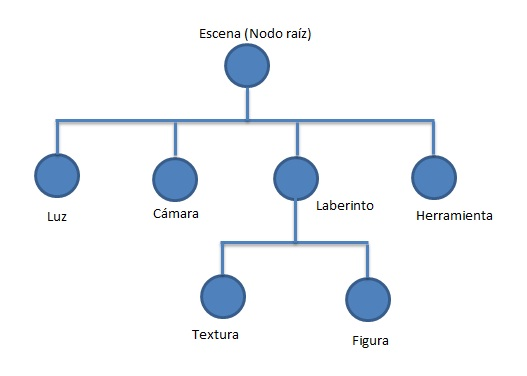
\includegraphics[width=11cm,height=8cm]{imag//nombredelaimagen.jpg}\\
	\caption{T�tulo de la imagen.}\label{fig01}
	\endcenter
\end{figure}


\subsection{Uso de llaves}
Es un ejemplo de como usar los diagramas de llaves
\begin{displaymath}
Tema Principal\left\lbrace
\begin{array}{lcr}
subtema1\\
subtema2 \left\lbrace 
	\begin{array}{lcr} 
		uno\\
		dos 
	\end{array} \right.\\
subtema3\\
ultimosubtema
\end{array} \right.
\end{displaymath} 

\section{Dos Figuras}

Ejemplo de insertar dos figuras (hacerlo bajo su propio riesgo... no muy recomendado)

\begin{figure}[htbp]
	\begin{minipage}{7cm}
		\centerline{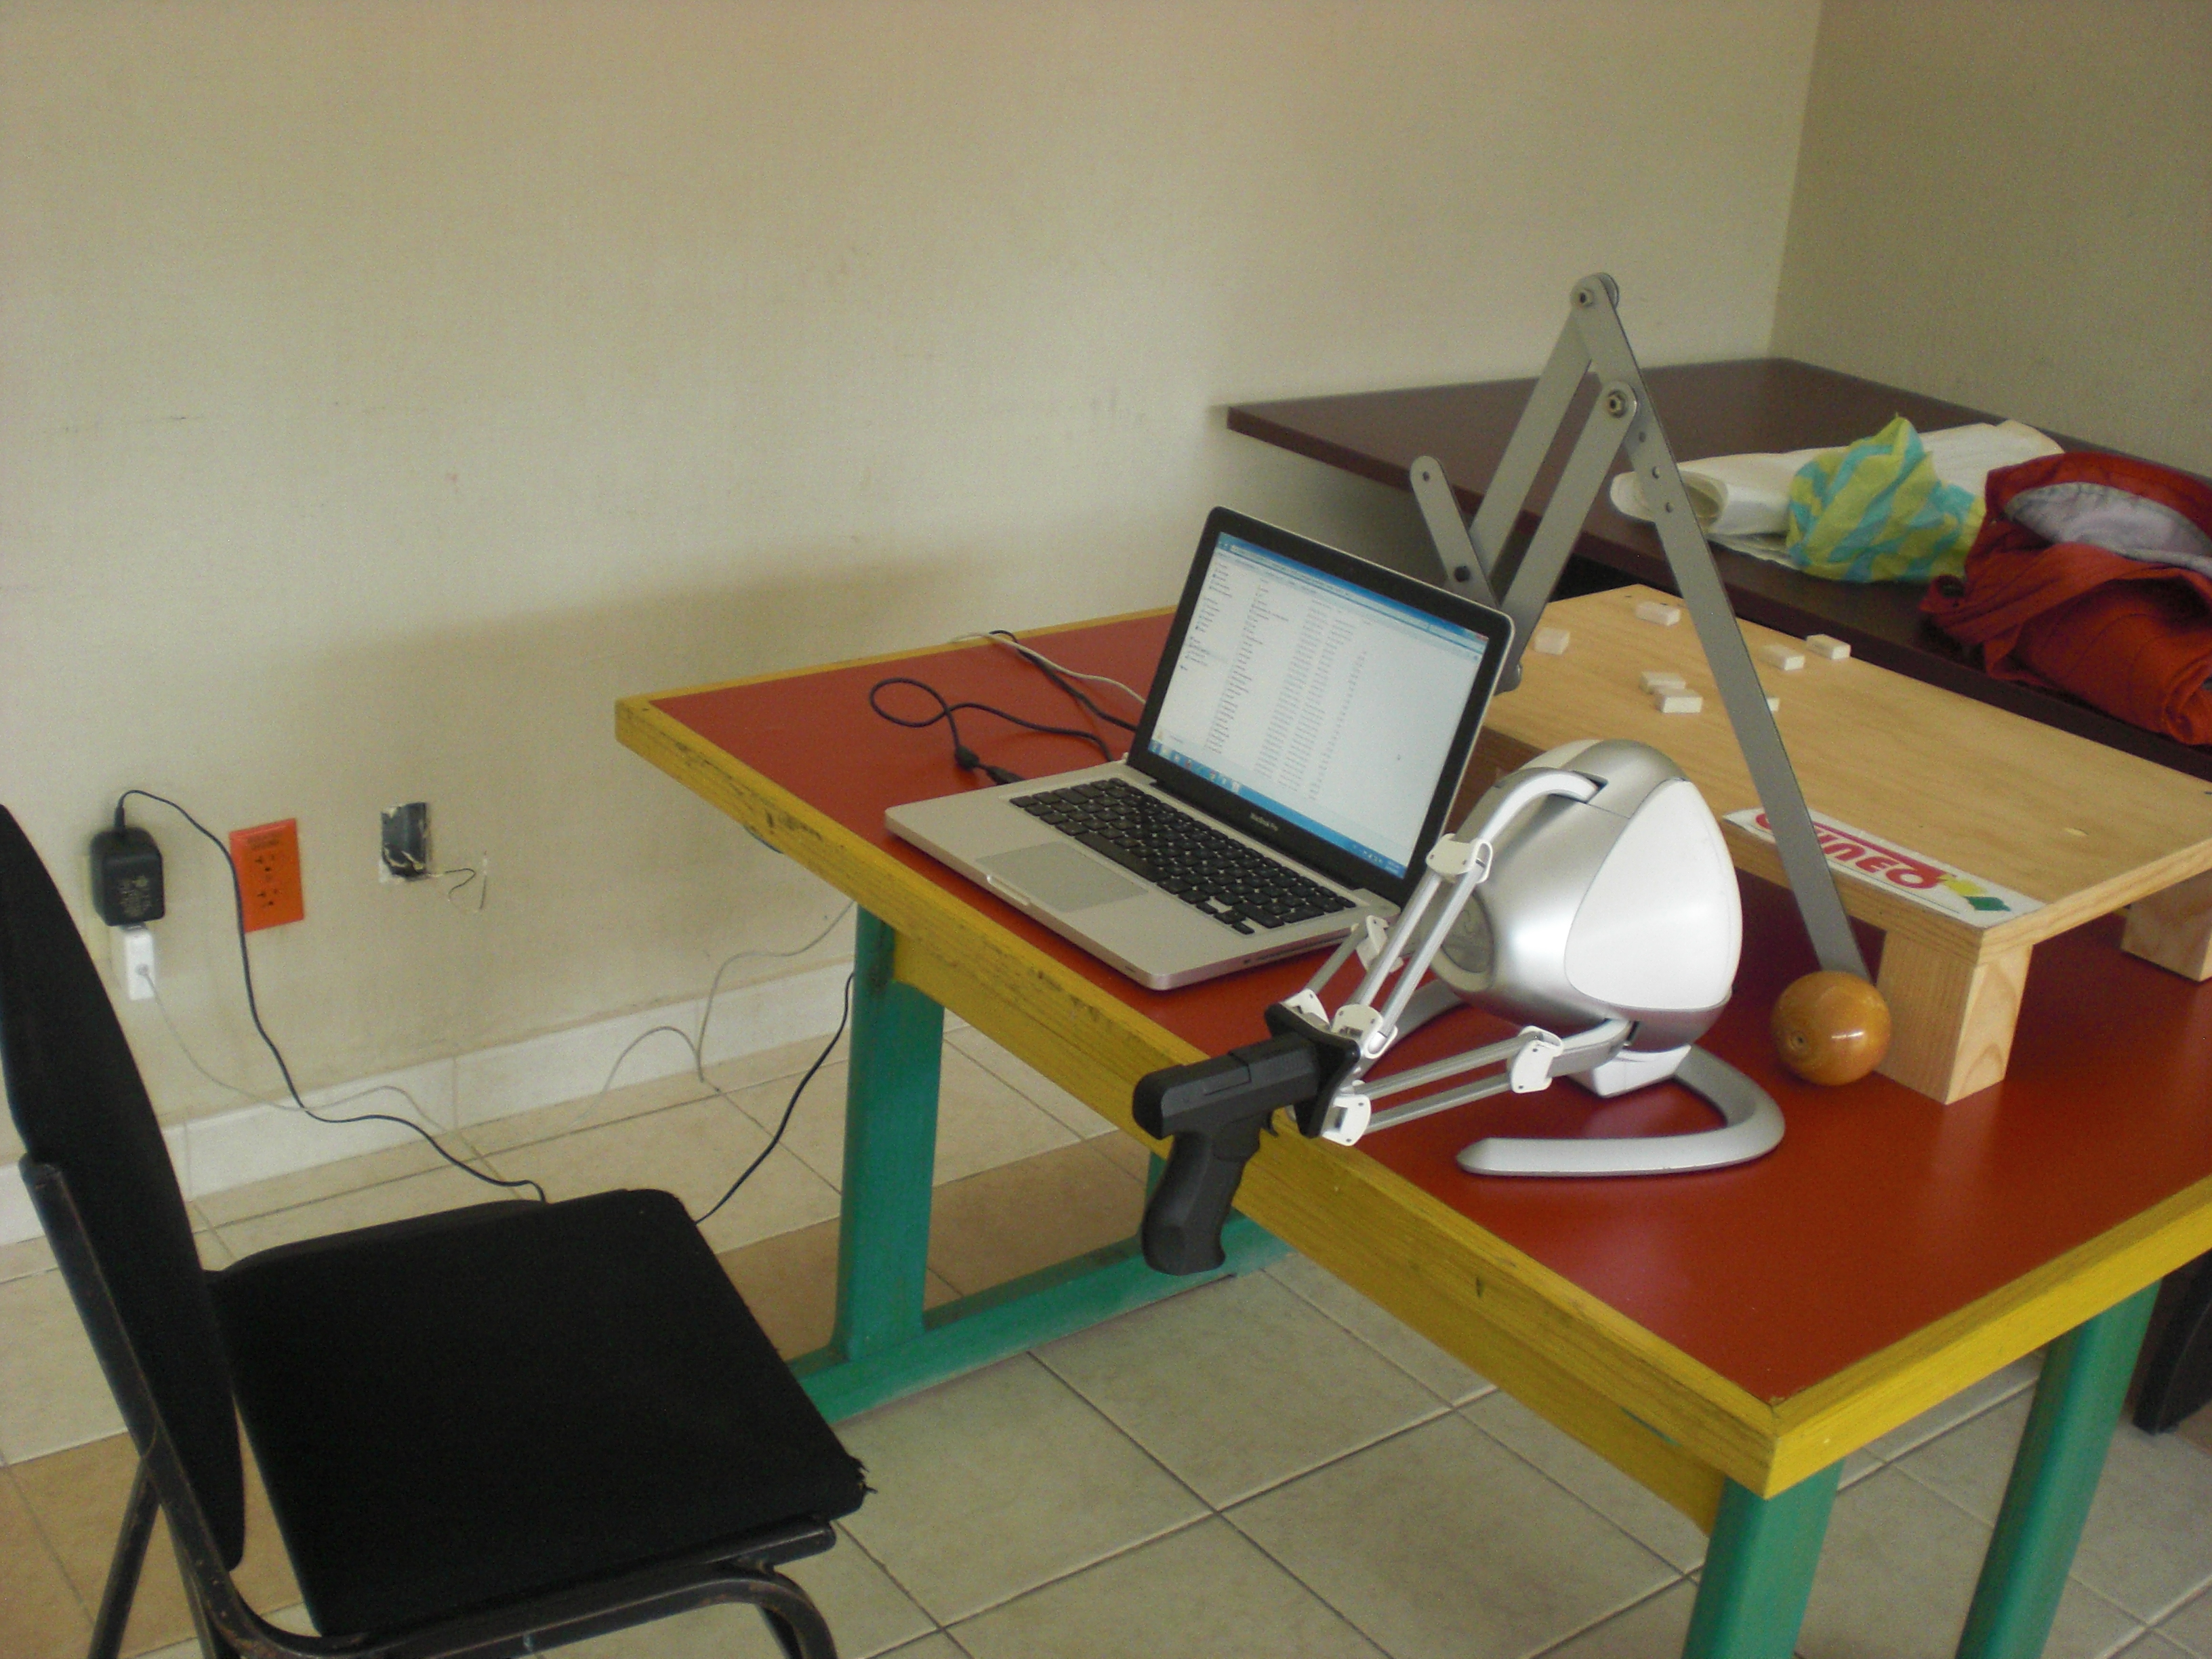
\includegraphics[height=5cm,width=7cm,angle=0]{imag//cree//Izquierda.jpg}}
		\vspace{0.5cm}
		\caption{T�tulo imagen izquierda.}\label{figIz}
	\end{minipage}\hspace{0.8cm}
	\begin{minipage}{7cm}
		\centerline{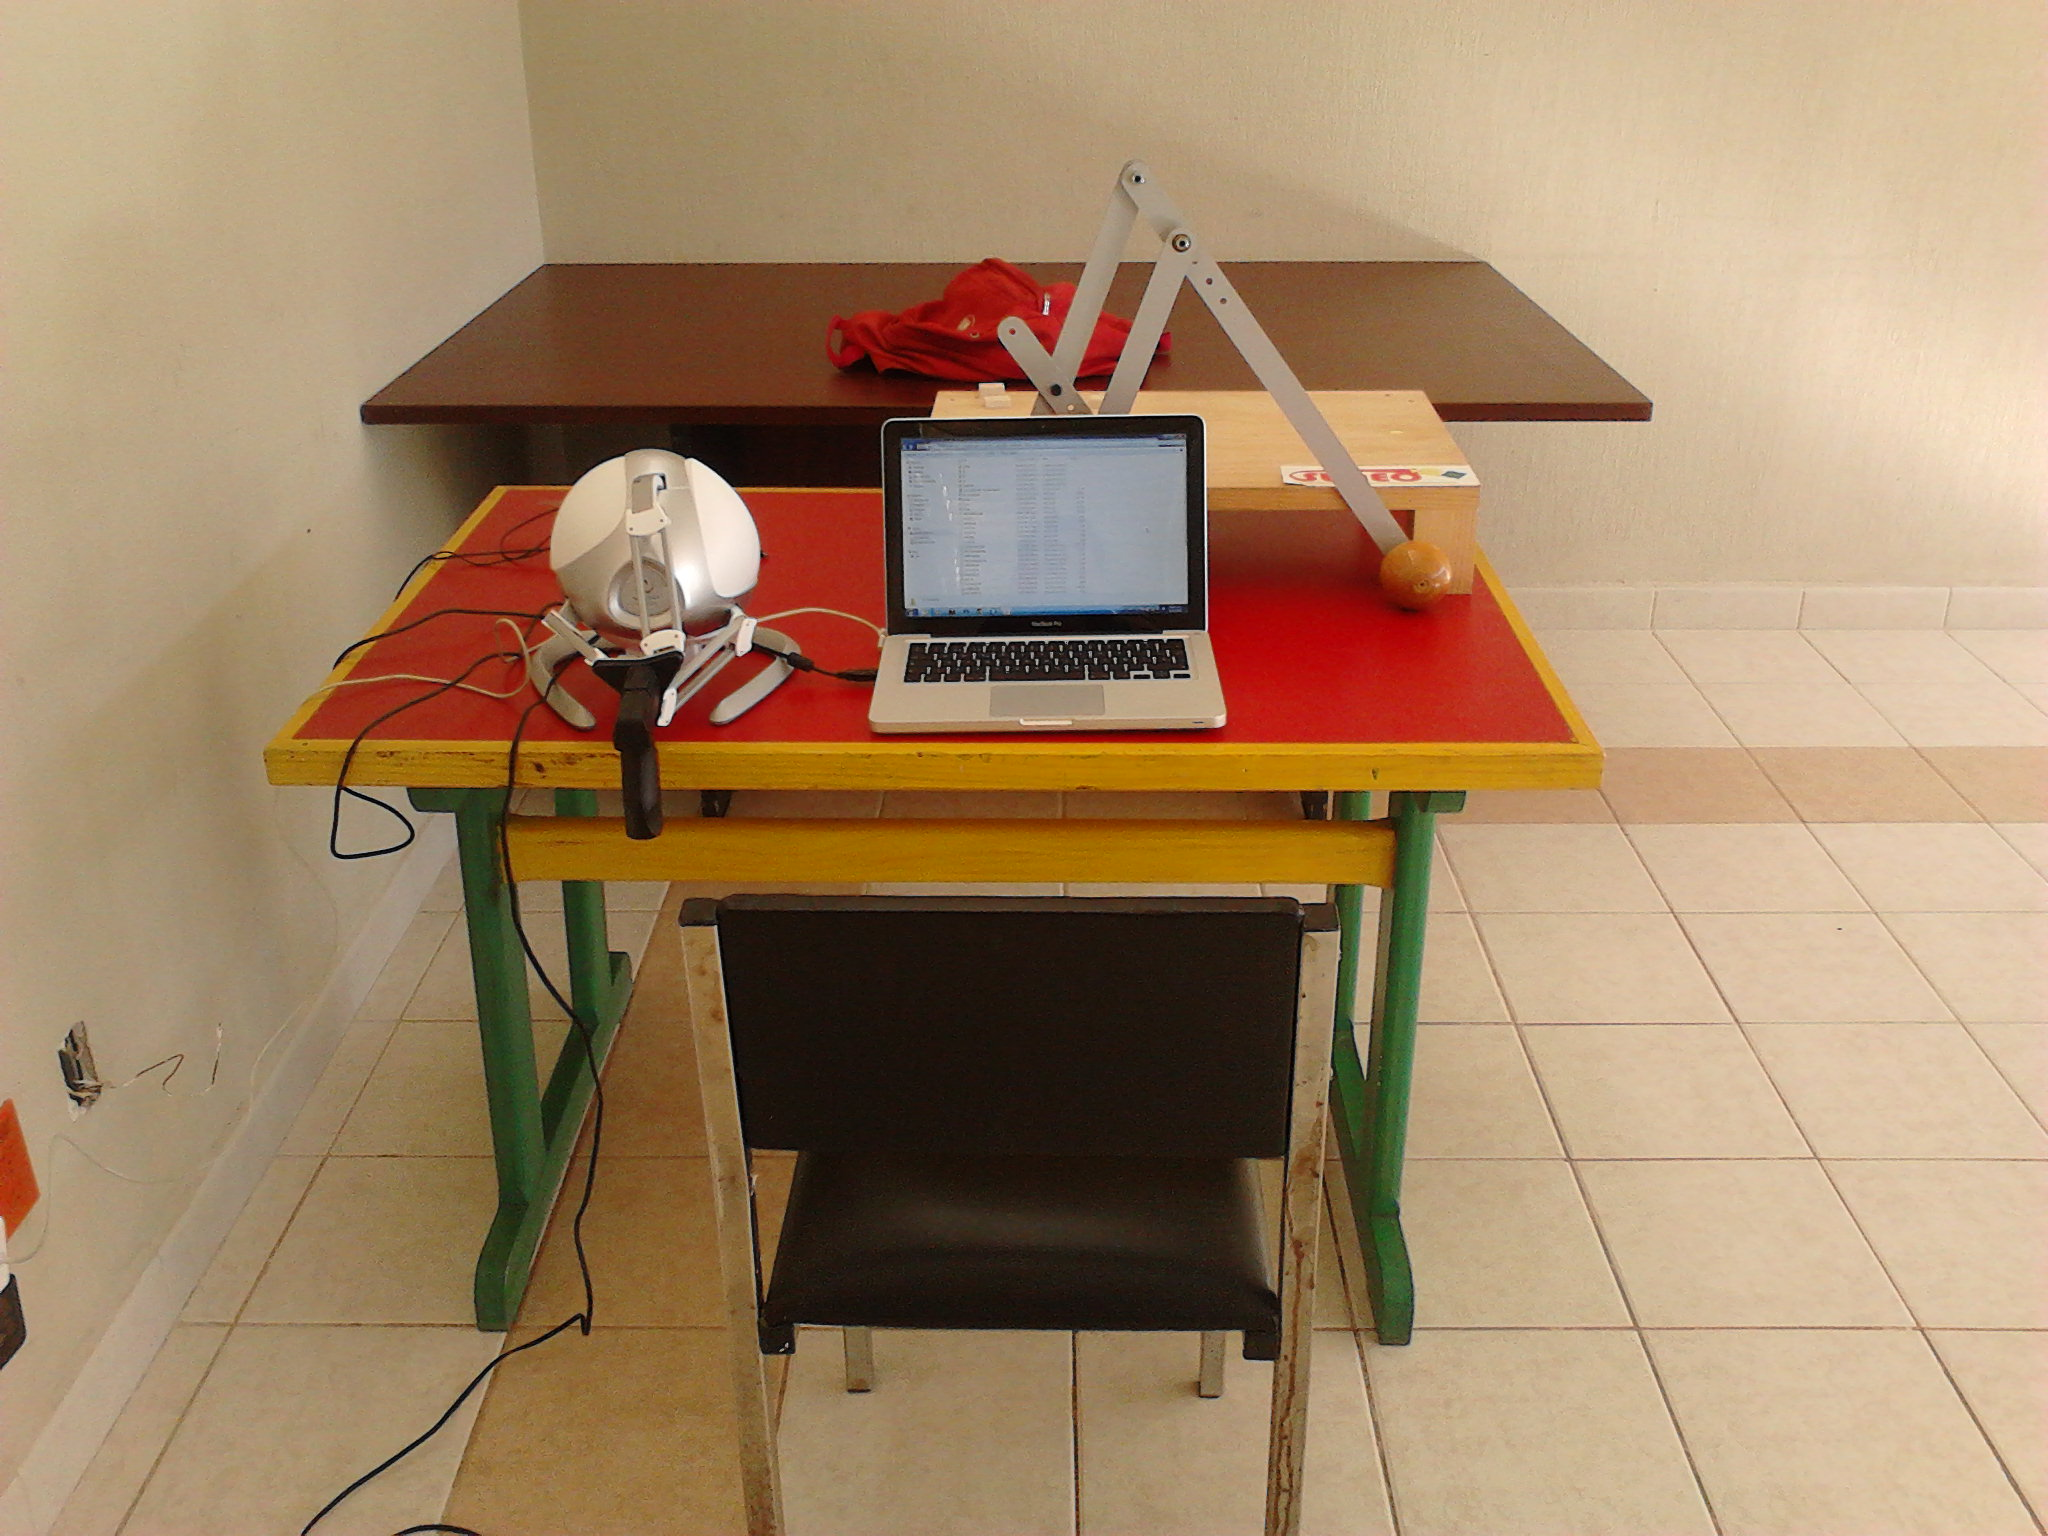
\includegraphics[height=5cm,width=7cm,angle=0]{imag//cree//Derecha.jpg}}
		\vspace{0.5cm}
		\caption{T�tulo imagen derecha.}\label{figDe}
	\end{minipage}
\end{figure}

A continuaci�n se muestra la forma de realizar un listado...

\begin{enumerate}
	\item Item 1
	\item Item 2
	\item Item 3
\end{enumerate}

Otra forma de enlistar..

\begin{enumerate}
	\item[a)] Item a
	\item[b)] Item b
	\item[c)] Item c
\end{enumerate}

Otro estilo.. 

\begin{itemize}
	\item Item a.1
	\item Item a.2
	\item Item a.3
\end{itemize}

\subsection{Ejemplos de Tablas}

\subsubsection{Insertar tabla a dos columnas}
Como se inserta la tabla \ref{tabla1} 
\begin{table}[h]
	\caption{Descripci�n de la tabla}\label{tabla1}
	\vspace{-0.5cm}
	\begin{center}
		\begin{tabular}{|p{5cm}|p{5cm}|}
			\hline
			Campo11 & Campo12 \\
			\hline
			Campo21 & Campo22\\
			\hline
			Campo31 & Campo32 \\
			\hline
		\end{tabular}
	\end{center}
\end{table}

\subsubsection{Insertar tabla a m�s columnas}

Como se inserta la tabla \ref{tabla2}

\begin{table}[htpb]
	\caption{Descripci�n de la tabla}\label{tabla2}
	\vspace{-0.5cm}
	\begin{center}
		\begin{tabular}{|p{3cm}|p{3cm}|p{3cm}|p{3cm}|}
			\hline
			Campo11 & Campo12 & Campo13 & Campo14 \\ \hline
			Campo21 & Campo22 & Campo23 & Campo24 \\ \hline
			Campo31 & Campo32 & Campo33 & Campo34 \\ \hline
		\end{tabular}
	\end{center}
\end{table}


\subsection{Otros formatos}

Las ecuaciones del pant�grafo est�n dadas por las ecuaciones:

\begin{equation}\label{eq1}
\lambda*AB=AE
\end{equation}
\begin{equation}\label{eq2}
\lambda*ED=EF
\end{equation}
\begin{equation}\label{eq3}
\lambda*AC=AF
\end{equation}
Donde $\lambda$ representa la escala de reproducci�n tal  que $\lambda>0$, y $\lambda\neq1$
determinando as�  que para el caso de la plataforma $\lambda=2$ considerando agregar 5cm de m�s al segmento EF
para colocar el sujetador final \cite{capitulo32}.


Para determinar el grupo de control se elabor� un cuestionario que fue aplicado a una muestra de poblaci�n de forma aleatoria (uso de verbatim).
\begin{verbatim}
Entrevista n�mero: _____________________

Edad: ______    Escolaridad: _______________
Estado civil: _____________
Ocupaci�n: ________________________________________________
La siguiente encuesta tiene como fin el establecer un grupo
de control  por lo que sus respuestas ser�n tratadas de for-
ma confidencial y la informaci�n que nos proporcione ser�
exclusivamente para la investigaci�n llevada a cabo.
Por tal motivo pedimos contestar con la mayor sinceridad
posible.

1.- �Usted consume bebidas alcoh�licas?
Si ____                         No_____
Si su respuesta fue "No", omita la siguiente pregunta
1.1	�Con que frecuencia usted consume bebidas alcoh�licas?
a)	Frecuentemente	b) a veces	c) solo en fiestas u ocasionalmente
2.- �sufre usted de hipertensi�n?
Si ____		         No____
3.- �Es usted zurdo o diestro?
____ Zurdo	        ___Diestro
4.- �Ha sufrido alg�n tipo de lesi�n en el brazo o en las manos (fracturas)?
SI____		        No_____
5.- �Ha tenido alg�n antecedente de par�lisis?
S�____		       No______
6.- �Ha sufrido ataques de epilepsia?
S�______		      No_____
7.- �Padece de artritis reumatoide?
S�___ 			No____
\end{verbatim}


Ejemplo de la codificaci�n de un algoritmo en C. Algoritmo Runge Kutta

\begin{lstlisting}

double RKS(double a)
{
double h, k1, k2, k4;

h=0.001;
k1=(a);
k2=(a+h/2.0);
k4=(a+h);
return (h*(k1+4*k2+k4)/6.0);

}
cVector3d RK(cVector3d t){
cVector3d s(RKS(t.x),RKS(t.y),RKS(t.z));
return s;
}
\end{lstlisting}

\cleardoublepage
\appendix
\cleardoublepage

\chapter{T�tulo del Ap�ndice}


\begin{lstlisting}
#include <assert.h>
#include <math.h>
#include <stdio.h>
#include <stdlib.h>
#include <string.h>
#include <sstream>
#include <cstdlib>
// DECLARACI�N DE CONSTANTES
//---------------------------------------------------------------------------
Registro *PRegistro=NULL;
// tama�o inicial (ancho / alto)
const int WINDOW_SIZE_W         = 600;
const int WINDOW_SIZE_H         = 600;
\\...
return (0);
}
\end{lstlisting}
\cleardoublepage
\bibliography{Bibliografia}
\bibliographystyle{apacite}
\end{document}
